\documentclass[14pt,a4paper,russian]{extreport}
\usepackage[utf8]{inputenc}
\usepackage[russian]{babel}
\usepackage{float}
\usepackage{ulem}
\usepackage{xcolor}
\usepackage{epigraph}
\usepackage{cmap} % для кодировки шрифтов в pdf
\usepackage[T2A]{fontenc}
\usepackage{pscyr}
\usepackage{indentfirst} % отделять первую строку раздела абзацным отступом тоже
\usepackage[textwidth=100, textsize=footnotesize]{todonotes}


% Добавляем гипертекстовое оглавление в PDF
\usepackage[
bookmarks=true, colorlinks=true, unicode=true,
urlcolor=black,linkcolor=black, anchorcolor=black,
citecolor=black, menucolor=black, filecolor=black,
]{hyperref}

\usepackage{graphicx}   % Пакет для включения рисунков
\usepackage{lscape}
\usepackage{booktabs}

% С такими оно полями оно работает по-умолчанию:
%\RequirePackage[left=20mm,right=10mm,top=20mm,bottom=20mm,headsep=0pt,includefoot]{geometry}
% Если вас тошнит от поля в 10мм --- увеличивайте до 20-ти, ну и про переплёт не забывайте:

\linespread{1.3} % полуторный интервал

% Пакет Tikz
\usepackage{dot2texi}
%\usepackage{dot2texi}
\usepackage{tikz}
\usetikzlibrary{shapes,arrows,positioning,shadows}

% Произвольная нумерация списков.
\usepackage{enumerate}

% ячейки в несколько строчек
\usepackage{multirow}

% itemize внутри tabular
\usepackage{paralist,array}
\usepackage{tabularx}

%\setlength{\parskip}{1ex plus0.5ex minus0.5ex} % разрыв между абзацами
\setlength{\parskip}{1ex} % разрыв между абзацами
\usepackage{blindtext}

% Центрирование подписей к плавающим окружениям
%\usepackage[justification=centering]{caption}

\usepackage{newfloat}

\renewcommand{\rmdefault}{ftm} % Times New Roman


% Загаловки

\usepackage{titlesec}
 
\titleformat{\chapter}[display]
    {\filcenter}
    {\MakeUppercase{\chaptertitlename} \thechapter}
    {8pt}
    {\bfseries}{}
 
\titleformat{\section}
    {\normalsize\bfseries}
    {\thesection}
    {1em}{}
 
\titleformat{\subsection}
    {\normalsize\bfseries}
    {\thesubsection}
    {1em}{}
 
% Настройка вертикальных и горизонтальных отступов
\titlespacing*{\chapter}{0pt}{-30pt}{8pt}
\titlespacing*{\section}{\parindent}{*4}{*4}
\titlespacing*{\subsection}{\parindent}{*4}{*4}


%Поля
\usepackage{geometry}
\geometry{left=3cm}
\geometry{right=1.5cm}
\geometry{top=2.4cm}
\geometry{bottom=2.4cm}

%Оглавления
\usepackage{tocloft}
\renewcommand{\cfttoctitlefont}{\hspace{0.38\textwidth} \bfseries\MakeUppercase}
\renewcommand{\cftbeforetoctitleskip}{-1em}
\renewcommand{\cftaftertoctitle}{\mbox{}\hfill \\ \mbox{}\hfill{\footnotesize Стр.}\vspace{-2.5em}}
\renewcommand{\cftchapfont}{\normalsize\bfseries \MakeUppercase{\chaptername} }
\renewcommand{\cftsecfont}{\hspace{31pt}}
\renewcommand{\cftsubsecfont}{\hspace{11pt}}
\renewcommand{\cftbeforechapskip}{1em}
\renewcommand{\cftparskip}{-1mm}
\renewcommand{\cftdotsep}{1}
\makeatletter
    \renewcommand{\@dotsep}{2}
    \newcommand{\l@likechapter}[2]{{\bfseries\@dottedtocline{0}{0pt}{0pt}{#1}{#2}}}
\makeatother
\setcounter{tocdepth}{2} % задать глубину оглавления — до subsection включительно

%Определение своей секции

\newcommand{\empline}{\mbox{}\newline}
\newcommand{\likechapterheading}[1]{ 
    \begin{center}
    \textbf{\MakeUppercase{#1}}
    \end{center}
    \empline}

\newcommand{\likechapter}[1]{    
    \likechapterheading{#1}    
    \addcontentsline{toc}{likechapter}{#1}}


%Работа с картинками

\usepackage[tableposition=top]{caption}
\usepackage{subcaption}
\DeclareCaptionLabelFormat{gostfigure}{Рисунок #2}
\DeclareCaptionLabelFormat{gosttable}{Таблица #2}
\DeclareCaptionLabelSeparator{gost}{~---~}
\captionsetup{labelsep=gost}
\captionsetup[figure]{labelformat=gostfigure}
\captionsetup[table]{labelformat=gosttable}
\renewcommand{\thesubfigure}{\asbuk{subfigure}}
% 8 Листинги

\usepackage{listings}

% Значения по умолчанию
\lstset{
  basicstyle= \footnotesize,
  breakatwhitespace=true,% разрыв строк только на whitespacce
  breaklines=true,       % переносить длинные строки
%   captionpos=b,          % подписи снизу -- вроде не надо
  inputencoding=koi8-r,
  numbers=left,          % нумерация слева
  numberstyle=\footnotesize,
  showspaces=false,      % показывать пробелы подчеркиваниями -- идиотизм 70-х годов
  showstringspaces=false,
  showtabs=false,        % и табы тоже
  stepnumber=1,
  tabsize=4,              % кому нужны табы по 8 символов?
  frame=single
}

% Стиль для псевдокода: строчки обычно короткие, поэтому размер шрифта побольше
\lstdefinestyle{pseudocode}{
  basicstyle=\small,
  keywordstyle=\color{black}\bfseries\underbar,
  language=Pseudocode,
  numberstyle=\footnotesize,
  commentstyle=\footnotesize\it
}

% Стиль для обычного кода: маленький шрифт
\lstdefinestyle{realcode}{
  basicstyle=\scriptsize,
  numberstyle=\footnotesize
}

% Стиль для коротких кусков обычного кода: средний шрифт
\lstdefinestyle{simplecode}{
  basicstyle=\footnotesize,
  numberstyle=\footnotesize
}

% Стиль для BNF
\lstdefinestyle{grammar}{
  basicstyle=\footnotesize,
  numberstyle=\footnotesize,
  stringstyle=\bfseries\ttfamily,
  language=BNF
}

% Определим свой язык для написания псевдокодов на основе Python
\lstdefinelanguage[]{Pseudocode}[]{Python}{
  morekeywords={each,empty,wait,do},% ключевые слова добавлять сюда
  morecomment=[s]{\{}{\}},% комменты {а-ля Pascal} смотрятся нагляднее
  literate=% а сюда добавлять операторы, которые хотите отображать как мат. символы
    {->}{\ensuremath{$\rightarrow$}~}2%
    {<-}{\ensuremath{$\leftarrow$}~}2%
    {:=}{\ensuremath{$\leftarrow$}~}2%
    {<--}{\ensuremath{$\Longleftarrow$}~}2%
}[keywords,comments]

% Свой язык для задания грамматик в BNF
\lstdefinelanguage[]{BNF}[]{}{
  morekeywords={},
  morecomment=[s]{@}{@},
  morestring=[b]",%
  literate=%
    {->}{\ensuremath{$\rightarrow$}~}2%
    {*}{\ensuremath{$^*$}~}2%
    {+}{\ensuremath{$^+$}~}2%
    {|}{\ensuremath{$|$}~}2%
}[keywords,comments,strings]

% Подписи к листингам на русском языке.
\renewcommand\lstlistingname{Листинг}
\renewcommand\lstlistlistingname{Листинги}

% Любимые команды
\newcommand{\Code}[1]{\textbf{#1}}

\newcommand{\SetTextInfo}[3]{
	\newcommand{\TextHeadline}{#1}
	\newcommand{\TextAutor}{#2}
	\newcommand{\TextDate}{#3}
}

\newcommand{\SetTextStatus}[1]{
	\newcommand{\TextStatus}{{#1}}
}

\newcommand{\PrintTextInfo}{
	\epigraph{\textbf{\TextHeadline} \\ \TextStatus}{Автор: \TextAutor\\ Дата: \TextDate}
}



%%%%%%%%%%%%%%%%%%%%%%%%%%%%%%%%%%%%%%%%%%%%%
% Задать заголовок документа, автора и дату %
% первый аргумент - заголовок, второй автора, трейти дата%
\SetTextInfo{Template}{Vlasov}{07.09.2019}
\SetTextStatus{Готов}

\begin{document}

\title{Методы оптимизации и оперативного планирования сборочных производств}

\maketitle

\tableofcontents %Создание оглавления
\section*{Введение}
\addcontentsline{toc}{chapter}{Введение}
Современные системы автоматизации производств глубоко интегрируются в реальные процессы. При этом интегрируются на уровне SCADA(Supervisory Control And Data Acquisition — диспетчерское управление и сбор данных) систем, на уровне сбора первичных данных, если система производства слабо автоматизирована, то интеграция происходит на уровне носимых устройств, систем распределения задач, а также систем исполнения процессов. 

Разрабатываемая система цифрового двойника, глубоко интегрированная в производственные процессы, представляет из себя не что иное, как кибер-физическую систему, которая на основе обратной связи относительно физического объекта принимает решение, анализирует его поведение и формирует управляющие воздействия. Более того, разрабатываемый модуль ориентирован на то, чтобы быть встроенным в качестве главного узла принятия решений в системе автоматизированного производства.

Глобальная цель такого рода разработок направлено на то, чтобы исключить менеджмент среднего уровня, заменив его алгоритмами. Оставить только менеджеров высокого уровня, которые будут принимать общее решения относительно в какое направление развивать производство, руководствуясь данными цифровых двойников для того, чтобы принятие решения не сводилась к персональным оценкам, а в них была объективность

\newpage

\textbf{Актуальность темы исследования.} Создание цифрового двойника производства зарекомендовала себя, как безопасный способ получение желаемого результата от реального объекта, не прибегаю к тестированию на реальном производстве. Методы моделирования и, в частности имитационного, постоянно модернизируются, чтобы достичь максимальной точности по отношению к моделируемым объектам.

\textbf{Степень теоретической разработанности темы.} Так как проблема актуальна, по данной тематике существуют большое количество публикаций. Данные публикации в целом сосредоточены на разработке новых подходов к моделированию производств, но также есть и обзорные исследования.

\textbf{Целью работы} является разработка гибридной имитационной модели, а также методов оптимизации поиска оперативного плана.

Для достижения данной цели были поставлены следующие задачи:

\begin{enumerate}
    \item [1)]обзор систем имитационного моделирования, подходов к реализации;
    \item [2)]разработка алгоритмов и методов имитационного моделирования;
    \item [3)]алгоритмы оптимизации оперативного плана, построенного на основе имитационной модели;
    \item [4)]алгоритмы оптимизации планирования конвейеризированных процессов.
\end{enumerate}







% \todo[inline, color=red]{2-3 страницы пока не понятно о чем???}
\chapter{Автоматизация производственного планирования}
\section{Развитие систем управления и планирования предприятием}
На сегодняшний день, в условиях серьезной конкуренции очень важно следить за всеми новинками технологического прогресса и своевременно внедрять в структуру производства.
Так организация предприятия напрямую влияет на эффективность производства. Основным направлением организацией предприятием в последнее время относят системы ИСУП, которые позволяют достичь следующих задач: выполнение планов производства, оптимизация производственного процесса, снижение издержек и повышение эффективности производства.

Данные системы начали появляться с развитием компьютерных технологий в начале 80-х годов. Одной из главных причин появления данных систем является нехватка административного, бухгалтерского и технического персонала, который обладал бы достаточной квалификацией для обработки информации предприятия, также стало понятно, что предприятия не могут позволять себе большие объемы материального запаса для производства продукции. Это привело к появлению систем планирования потребности в ресурсах. Первым шагом в этом направлении был MRP (Materials Resource Planning), который включал только материалы планирования для производства \cite{MRP}.

Основной концепция MPR заключается в минимизации затрат связанных с запасами, а также расчет сколько и в какие сроки необходимо произвести конечный продукт. 

Недостатками данной системы является, то что при расчете потребностей в материалах не учитываются производственные мощности, их загрузки, трудозатраты и т.д. 

Логическим продолжением MPR системы стала система MPR 2, которая в отличие от предшественника учитывала финансовую составляющую предприятия, а также охватывала более широкий охват ресурсов. Это позволило компаниям иметь более интегрированную бизнес-систему, которая выводила требования к материалам и мощности, связанные с желаемым планом операций, позволяла вводить подробные данные о деятельности, переводить все это в финансовый отчет и предложить план действий для решения тех вопросов, которые были не в соответствии с желаемым планом.

К началу 1990-х годов постоянные улучшения в технологии позволили расширить MRP II, включив в него все планирование ресурсов для всего предприятия. Такие области, как дизайн продукта, хранение информации, планирование мощностей, системы связи, управление персоналом, финансы и управление проектами, теперь могут быть включены в план. Отсюда и термин ERP (Enterprise Resource Planning). И ERP можно использовать не только в производственных компаниях, но и в любой компании, которая хочет повысить конкурентоспособность путем наиболее эффективного использования всех своих активов, включая информацию \cite{ptak_schragenheim_2004} [23,25].

Разрабатываемое программное обеспечение принадлежит к классу ERP-систем. Многие современные ERP-систем разработаны по модульному принципу, поэтому существует возможность выбирать и внедрять только те модули, которые необходимы клиенту. 

В данной работе рассматривается одна из частей ERP систем,отвечающая за сопоставление конструкторских и технологических спецификаций, определяющих состав конечного продукта и ресурсов предприятия. На основании данного сопоставления построение плана производственного процесса, учитывающие ограничения предприятия, а также реализация частных математических моделей. Математические модели призваны оптимизировать производственный процесс в зависимости от специфики\footnote{Примером такой специфики является конвейеризированное предприятие.} предприятия.

\section{Функции систем управления и планирование предприятием}

Информационно - управляющая система предприятием(ИСУП) способна эффективно поддерживать производство в соответствии с расписанием посредством анализа данных и простой интеграции на предприятии. Хотя система не может самостоятельно управлять производственным оборудованием, она все же способна поддерживать постоянный поток материалов по всей цепочке поставок с помощью возможностей принятия решений. Различные функции системы ИСУП включают в себя следующее:

\begin{itemize}
    \item высокая точность соблюдения сроков (и поставка заданных количеств);
    \item оптимальная загрузка производственных мощностей;
    \item короткие производственные циклы;
    \item минимальный уровень капиталовложения;
    \item поддержание необходимого уровня складских запасов и материалов на производстве;
    \item высокая гибкость;
    \item минимизация расходов.
\end{itemize}

В следующем разделе приведены источники роста эффективности, используемые ИСУП для достижения оптимального результата. 

\section{Источники роста эффективности}

В промышленности есть огромные неиспользованные резервы роста производительности труда. Они могут быть подразделены на резервы снижения трудоемкости продукции и резервы рабочего времени.( см. рисунок \ref{ris:reserve1})

Резервы снижения трудоемкости выявляются и реализуются в виде экономии рабочего времени, затрачиваемого непосредственно на выполнение рабочих операций.

Резервы фонда рабочего времени реализуются путем повышения эффективности использования рабочего процесса для данного коллектива в течение определенного планового периода\cite{Lenin}. 


\begin{figure}[H]
    \center{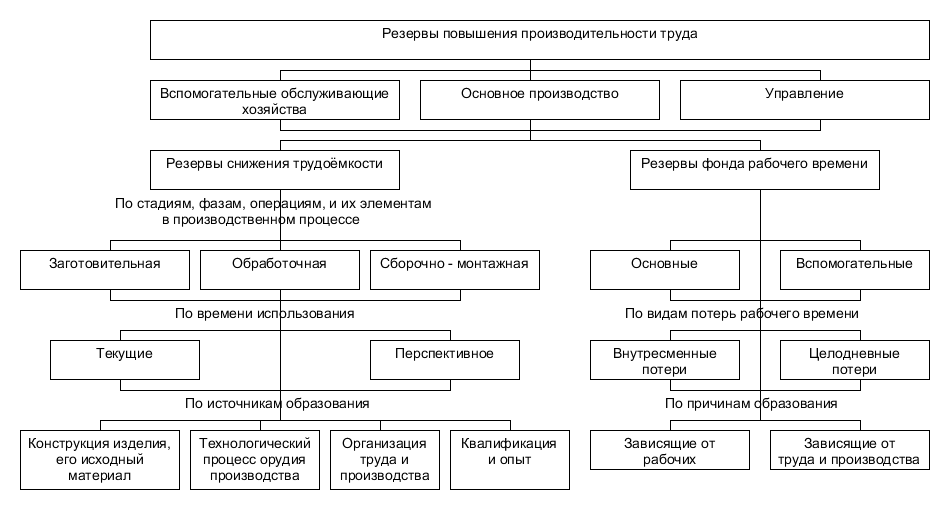
\includegraphics[width=1\linewidth]{fig/reserve1.png}}
    \caption{Резервы роста производительности труда}
    \label{ris:reserve1}
\end{figure}

Исходя из информации представленной на рисунке \ref{ris:reserve1}, можно сделать вывод, что повышение эффективности производства может быть достигнуто, как и грамотной организацией резервов рабочего времени, так и путем пересмотра техники выполнения рабочих операций, но не все резервы повышения производительности можно решить в рамках ИУС. К таким резервам относится конструктивные особенности изделия, так как требуют изменения исходной конструкции продукта, что не является задачей ИУС. 


\section{Обзор существующих решений}
\indent Сегодня, чтобы сохранять конкурентоспособность, предприятиям необходимо развивать и внедрять системы управления и планирования производственных процессов. 
Актуальным направлением, ориентированным на решение этой задачи, является разработка СПП, которая должна обеспечивать решение следующих задач: исполнения планов производства и целевых показателей, оптимизации операционной деятельности, снижения затрат и повышения эффективности производства.\\
\indent Производственное планирование — это систематический, структурированный, направленный на достижение поставленной задачи процесс планирования промышленного предприятия, состоящий из отдельных, иерархически распределенных этапов, осуществляемый с помощью специальных методов и инструментов, начиная с момента появления замысла и заканчивая запуском производства \cite{mulBook}.
Производственное планирование может также включать в себя корректирующие мероприятия в процессе эксплуатации. Планирование промышленного предприятия может основываться на различных целях и задачах, охватывать самые разные проектные ситуации.\\
\indent В процессе планирования используется ряд инструментов и программных компонент, которые поддерживают реализацию метода планирования \cite{lodonBook}.
Говоря в общем, это программные средства (прикладные программы), которые применяются пользователями на персональных компьютерах в различных фазах планирования жизненного цикла промышленного предприятия.
К основным инструментам планирования относятся: APS/SCM; САР; АСУП. 
Ниже даны подробные описания данных инструментариев \cite{oliriBook}.\\
\indent APS/SCM (системы синхронного планирования, системы управления логической цепочкой) поддерживают расчеты, эксплуатацию и оптимизацию логистических цепочек. 
Особые свойства логистической цепочки получаются благодаря взаимодействию участников. 
Важная роль отводится структуре логистических цепочек, соответствующих рынку, а также координации и интеграции всех индивидуальных действий.\\
\indent САР (система автоматизированного регулирования) характеризует область компьютеризованного планирования работы. 
При этом используется система электронной обработки данных для создания рабочего графика, выбора эксплуатационных средств, создания указаний по изготовлению и монтажу, а также программирования для ЧПУ.\\
\indent АСУП (САМ — автоматическая система управления производством) включает в себя компьютерное техническое управление и контроль над производственными линиями и эксплуатационными средствами при проведении производства, т.е. прямое управление обрабатывающими и перерабатывающими машинами, устройствами манипуляции, транспортировки, перегрузки и хранения, а кратко — техническое управление всеми устройствами потоковых систем \cite{gibBook}.\\
\indent Наиболее распространенными программными продуктами, предназначенными для планирования производственных процессов являются «1С:Предприятие» и «SAP R/3»: первый является наиболее распространенным на российском рынке, второй, в свою очередь, широко используется за рубежом. 
На примере этих, зарекомендовавших себя с положительной стороны, продуктов проведем анализ системных компонент и сравним их место в архитектуре систем.

\subsection{«1С: Предприятие 8.0»}

\indent Комплекс программ «1С: Предприятие 8.0» состоит из технологической платформы и прикладных компонентов, которые создаются на основе платформы и предназначены для автоматизации деятельности предприятий. 
Технологическая платформа не является готовым программным продуктом, предназначенным для внедрения на предприятие, вместо нее обычно применяют одну или несколько компонентов, разработанных на этой платформе. 
Данное решение делает возможным автоматизировать различные виды деятельности, применяя единую основную технологическую платформу.
\indent Система «1С: Предприятие 8.0» использует следующие основные компоненты:

\begin{itemize}
	\item «Управление торговлей»;
	\item «Управление персоналом»;
	\item «Управление производственным предприятием»;
	\item «Управление складом»;
	\item «Управленческий учет и расчет себестоимости».
\end{itemize}

\indent Наиболее интересными для рассмотрения являются компоненты «Управление персоналом» и «Управление производственным предприятием», поскольку их реализация является ключевой с точки зрения планирования деятельности предприятия и не имеет сегодня строгой математической формализации, чем отличаются компоненты, связанные с экономическим анализом деятельности.\\
\indent Компонент «1С: Предприятие 8.0. Управление персоналом» позволяет эффективно управлять кадровыми процессами в следующих областях: планирование потребностей в персонале; обеспечение организации новыми кадрами; эффективное планирование занятости персонала; кадровый учет и анализ персонала; управление персоналом.\\
\indent Компонент «Управление производственным предприятием» предназначена для автоматизации процессов управления и учета производственном предприятии.
Это позволяет создать единую информационную систему для управления различными сторонами деятельности предприятия.\\
\indent В платформе «1С: Предприятие 8.0» заложен ряд подходов, которые формируют основную концепцию разработки типовых компонентов. 
Эти подходы предназначены для максимального сближения технологических возможностей с бизнес-процессами разработки и интеграции прикладных решений.
Важными моментами, которые следует отметить, являются: изоляция разработчика от технологических деталей, алгоритмическое программирование конкретной бизнес-логики приложения, использование собственной модели базы данных и гибкость прикладных решений без их доработки.\\
\indent Механизм обмена данными, используемый в технологической платформе «1С: Предприятие 8.0», позволяет создавать территориально распределенные информационные системы на основе баз данных «1С: Предприятия 8.0», и использовать другие информационных систем, не относящиеся к «1С: Предприятии 8.0».
Например, можно организовать работу главного офиса, филиалов и складов предприятия в одной базе данных, или обеспечить взаимодействие базы данных «1С: Предприятия 8.0» с существующей базой данных «Oracle».\\
\indent Технологическая платформа «1С: Предприятие 8.0» предоставляет средства разработки, с помощью которых создаются новые или модифицируют существующие прикладные решения.
Этот инструмент разработки называется «конфигуратор».
Благодаря тому, что он поставляется со стандартным пакетом «1С: Предприятия 8.0», то пользователь может свободно разработать или модифицировать прикладное решение (адаптировать его под себя), возможно, с привлечением сторонних специалистов.\\
\indent Среди преимуществ данной системы можно выделить:

\begin{itemize}
	\item открытость системы;
	\item регулярные программные обновления;
	\item широкие функциональные возможности системы.
\end{itemize}


\indent Однако необходимо отметить, что подходы «1С: Предприятия» ориентированы на решение проблем автоматизации бухгалтерского и организационного управления предприятием.
Использование проблемно-ориентированных объектов позволяет разработчику решать задачи по складского, бухгалтерского, управленческого учета, расчетам заработной платы, анализа данных и управлению бизнес-процессами. 
Однако области экономического и бухгалтерское учета характеризуются высокой степенью математического формализма и их реализация происходит с относительно малыми трудозатратами, тогда как компоненты планирования и производственного расписания сегодня являются актуальными направлением для исследований и прикладной разработки.

\subsection{«SAP R/3»}

\indent Система «SAP R/3» предоставляет собой набор разноплановых инструментов, направленных на повышение эффективности производственного процесса, увеличение экономической стабильности, автоматизацию процессов планирования.
Она дает возможность интегрировать инновационные подходы централизованного планирования и управления, и повысить качество управления на разных организационных уровнях предприятий.\\
\indent «SAP R/3» является многомодульной системой, где каждый отдельный модуль предназначен, для решения специализированной задачи процесса предприятия, взаимодействие между ними происходит в режиме реального времени. 
Наибольший интерес для рассмотрения снова представляют компоненты, не имеющие прямого отношение к бухгалтерской и экономической деятельности предприятия - модуль PP; модуль HR; модуль BC.\\
\indent Модуль PP (планирование производства) дает возможность организовать управление и планирование производством предприятием.
Модуль PP реализует следующие функции: формирование спецификаций, создание технологических карт, управление производственными площадками, планирование сбыта, планирование потребности в материалах, управление производственными заказами, планирование затрат на изготовление изделие, учет затрат производственных процессов, планирование производственной деятельностью, управление серийным производством, систему, планирование автоматизированного производства.\\
\indent Модуль HR (управление персоналом) решает задачи планирования и управления работой персонала. 
Ключевые элементы: администрирование персонала, расчет данных для вычисления заработной платы, сбор и анализ данных о рабочем времени, учет командировочных расходов, создание информационной модели внутренней структуры компании.\\
\indent Модуль BC (базовый модуль) предназначен для интеграции в систему «SAP R/3» всех отдельных прикладных модулей и обеспечивает независимость от аппаратной платформы. 
Модуль BC позволяет организовать работу c многоуровневой распределенной архитектуре клиент-сервер. 
Система «SAP R/3» работает на серверах UNIX, AS/400, Windows NT, S/390 и с различными СУБД (Informix, Oracle, Microsoft SQL Server, DB2). 
Пользователи могут работать в среде Windows, OSF/Motif, OS/2 или Macintosh \cite{mazBook}.\\
\indent На данный момент система «SAP R/3» является наиболее распространенной системой управления предприятием. 
Благодаря тому, что она является модульной системой, ее можно настроить в соответствии с конкретными потребностями отдельного предприятия. 
Степень технического уровня системы определяется возможностью ее перенастройки без необходимости переписывать программный код. 
Эта опция «SAP R/3» также позволяет занимать ведущее место в мире в системе управления.\\
\indent С помощью инструментов управления, включенных в систему «SAP R/3», можно реализовывать задачи мониторинга и анализа, без дополнительного программирования, следующие способы:

\begin{itemize}
	\item мониторинг БД; 
	\item мониторинг операционной системы сервера; 
	\item мониторинг коммуникаций;
	\item мониторинг и управление сервером приложений:
	\begin{itemize}
		\item формирование и запуск новой конфигурация ядра R/3; 
		\item снятие и редактирование текущей конфигурации ядра R/3; 
		\item формирование временного графика в зависимости от нагрузки (например, в ночное время можно увеличивать количество процессов, отвечающих за фоновые задания); 
		\item управление системой архивирования; 
		\item управление текущими пользователями, процессами. 
	\end{itemize}
\end{itemize}

\indent Многоуровневая клиент-серверная архитектура позволяет разделять задачи, ориентированные на пользователя задачи управления данными. 
В версии 3.0 системы «SAP R/3» SAP AG были расширены возможности решения для взаимодействия с другими приложениями и расширены возможности распределения операций «SAP R/3» в масштабируемой компьютерной структуре. 
Технология внедрения «SAP R/3» основана на многоуровневой архитектуре с использованием программного обеспечения среднего уровня. 
Между тем, промежуточное ПО отделяет пользовательские приложения от аппаратного и программного обеспечения, с другой стороны, решает проблему взаимодействия программных приложений и аппаратным обеспечением. 
В «SAP R/3» SAP Basis функционирует как промежуточное программное обеспечение \cite{mazBook}.\\
\indent Основные данные — это информация, которая хранится в базе данных, достаточно долгий промежуток времени. 
К ним относятся такие данные как: информация о кредиторов, поставщиках, материалах и счета. 
Основные данные создаются централизованно и доступны для всех приложений. 
Например, они включают данные клиента, которые используются в заявках, поставках, выставления счетов и платежей. 
Запись основных данных клиента может быть присвоена следующим организационным единицам: балансовая единица, сбытовая организация, канал сбыта, сектор.\\
\indent Основная запись материала является центральным объектом данных системы «SAP R/3». 
Она включает в себя: сырье; оборудование; расходные материалы; полуфабрикаты; продукты; вспомогательное производственное оборудование и инструменты. 
Она является главным источником данных предприятия и используется всеми компонентами логистической системы SAP. 
Благодаря объединению всех данных материалов в единый объект базы данных устраняются проблемы избыточности данных. 
Сохранённые данные могут использоваться во всех областях, такими как закупки, контроль запасов, планирование потребностей в материалах, проверка счетов.\\
\indent Данные, хранящиеся в основной записи материала необходимы логистическому модулю системы для решения следующих задач: обработки запасов на поставку; обновления движения материалов и инвентаризационной обработки; проводки счетов; обработки клиентских заказов; планирования потребностей и календарного планирования. 
Структурная логика поставщика и клиента также применяется к основной записи материала. 
При оформлении заказа для клиентов необходимо учитывать: согласование о перевозки, условия доставки, оплаты и т.д. 
Данные, необходимые для таких операций, дублируются из основной записи делового партнера, чтобы исключить необходимость повторного ввода информации о каждой транзакции. 
В основной записи материала могут одновременно храниться данные, обработанные во время ввода заказа, например, цену за единицу цены товара, запасы на другом складе и т.д. 
Этот принцип полезен для обработки данных в каждой основной записи, связанной с выполнением операции.\\
\indent Для каждой транзакции необходимо присваивать соответствующую организационную единицу. 
Присвоение структуре предприятия в документе генерируется в дополнение к данным, доступным по клиенту и материалу. 
Поэтому документ, созданный при помощи транзакции, содержит все основные данные из организационных единиц \cite{gehBook}.\\
\indent Среди достоинств данной системы можно выделить:

\begin{itemize}
	\item прозрачность деятельность предприятия;
	\item повышение оборотов товарно-материальных запасов;
	\item сокращение персонала управления;
	\item единые стандарты управления.
\end{itemize}

\indent К недостаткам относятся:

\begin{itemize}
	\item требуется высокий уровень подготовки персонала;
	\item сложность интеграции;
	\item большие финансовые вложения.
\end{itemize}


\section{Обзор методов планирования производственных процессов.}

В данном разделе приведен перечень методов моделирования объектов и процессов.

% Please add the following required packages to your document preamble:
% \usepackage{graphicx}
% \renewcommand{\arraystretch}{1.8}
% \begin{table}[H]
%     \centering
%     \resizebox{\textwidth}{!}{%
%     \begin{tabular}{|c|c|c|c|c|}
%     \hline
%     Метод & Описание & \begin{tabular}[c]{@{}c@{}}Область\\ применения\end{tabular} & \begin{tabular}[c]{@{}c@{}}Достоинства \\ метода\end{tabular} & \begin{tabular}[c]{@{}c@{}}Недостатки \\ метода\end{tabular} \\ \hline
%     Математический & \begin{tabular}[c]{@{}c@{}}Составление математического \\ эквивалента процесса\\ или объекта, отражающий \\ его основные свойства\end{tabular} & \begin{tabular}[c]{@{}c@{}}Любые процессы и объекты, \\ поддающи­еся математическому \\ описанию\end{tabular} & \begin{tabular}[c]{@{}c@{}}Широкая область \\ применения\end{tabular} & \begin{tabular}[c]{@{}c@{}}Достаточно сложно \\ построить модель,\\ адекватно учитывающую \\ все факторы\end{tabular} \\ \hline
%     Статический & \begin{tabular}[c]{@{}c@{}}Модель основывается на \\ выявленных статических \\ закономерностях\end{tabular} & \begin{tabular}[c]{@{}c@{}}Процессы, по которым можно \\ собрать массив \\ статических данных\end{tabular} & \begin{tabular}[c]{@{}c@{}}При наличии качественных \\ данных метод точен \\ и, при использовании \\ специализированного \\ ПО, прост в применении.\end{tabular} & \begin{tabular}[c]{@{}c@{}}Большие требования \\ к статическим данным\end{tabular} \\ \hline
%     \begin{tabular}[c]{@{}c@{}}Экономико-\\ математический\end{tabular} & \begin{tabular}[c]{@{}c@{}}Раздел включает в \\ себя методы для \\ решения экономических \\ задач\end{tabular} & Экономические процессы & \begin{tabular}[c]{@{}c@{}}Метод способен \\ моделировать \\ экономические \\ процессы\end{tabular} &  \\ \hline
%     Имитационный & \begin{tabular}[c]{@{}c@{}}Изучаемая система\\  заменяется моделью, с\\  достаточной точностью\\  описывающей реальную\\  систему, с ней проводятся\\  эксперименты с целью\\  получения информации.\end{tabular} & \begin{tabular}[c]{@{}c@{}}Метод используется\\  когда дорого\\  или невозможно\\  использовать реальную\\  модель и/или\\  аналитическую модель\end{tabular} & \begin{tabular}[c]{@{}c@{}}Создается максимально\\  приближенная модель,\\  можно управлять\\  временем системы\\  и другими\\  её характеристиками.\end{tabular} & \begin{tabular}[c]{@{}c@{}}Сложность описания \\ всех условий\\  и требования\\  вычислительной \\ мощности.\end{tabular} \\ \hline
%     Физический & \begin{tabular}[c]{@{}c@{}}Экспериментальное\\  моделирование, \\ основанное\\  на физическом \\ подобии уменьшенной\\  в размерах модели.\end{tabular} & \begin{tabular}[c]{@{}c@{}}Применяется при \\ невозможности \\ применения аналитического\\  метода или воспроизведения\\  в реальном размере.\end{tabular} & \begin{tabular}[c]{@{}c@{}}Область применения,\\  недоступная другим\\  методам\end{tabular} & \begin{tabular}[c]{@{}c@{}}Метод может\\ дать надёжные\\  результаты лишь\\  при соблюдении\\  физического подобия\\  модели.\end{tabular} \\ \hline
%     \end{tabular}%
%     }
%     \end{table}

\subsubsection*{Математический}
\textbf{Описание.} Составление математического эквивалента процесса или объекта, отражающий его основные свойства.

\textbf{Область применения.} Любые процессы и объекты, поддающиеся математическому описанию.

\textbf{Достоинства метода.} Широкая область применения.

\textbf{Недостатки метода.} Достаточно сложно построить модель, адекватно учитывающую все факторы.

\subsubsection*{Статический}
\textbf{Описание.} Модель основывается на выявленных статических закономерностях.

\textbf{Область применения.} Процессы, по которым можно собрать массив статических данных.

\textbf{Достоинства метода.} При наличии качественных данных метод точен и, при использовании специализированного ПО, прост в применении.

\textbf{Недостатки метода.} Большие требования к статическим данным.
\subsubsection*{Экономико-математический}
\textbf{Описание.} Раздел включает в себя методы для решения экономических задач.

\textbf{Область применения.} Экономические процессы.

\textbf{Достоинства метода.} Метод способен моделировать экономические процессы.

\subsubsection*{Имитационный}
\textbf{Описание.} Изучаемая система заменяется моделью, с достаточной точностью описывающей реальную систему, с ней проводятся эксперименты с целью получения информации.

\textbf{Область применения.} Метод используется когда дорого или невозможно использовать реальную модель и/или аналитическую модель.

\textbf{Достоинства метода.} Создается максимально приближенная модель, можно управлять временем системы и другими её характеристиками.

\textbf{Недостатки метода.} Сложность описания всех условий и требования вычислительной мощности.

\subsubsection*{Физический}
\textbf{Описание.} Экспериментальное моделирование, основанное на физическом подобии уменьшенной в размерах модели.

\textbf{Область применения.} Применяется при невозможности применения аналитического метода или воспроизведения в реальном размере.

\textbf{Достоинства метода.} Область применения, недоступная другим методам.

\textbf{Недостатки метода.} Метод может дать надёжные результаты лишь при соблюдении физического подобия модели.

Для задач моделирования сложных, сборочных производств больше всего подходит метод имитационного моделирования, так как эксперементировать с реальным объектом экономически нецелесообразно, а также невозможно учесть все зависимости, что усложняет процесс аналитического моделирования.

\section{Обзор подходов к имитационному моделированию}

В прошлом производственные инструменты моделирования классифицировались как языки или симуляторы. \cite{Velazco} Языки были очень гибкими инструментами, но довольно сложными в использовании менеджерами и слишком трудоемкими. Симуляторы были более удобными для пользователя, но они шли с довольно жесткими шаблонами, которые недостаточно адаптировались к быстро меняющимся технологиям производства. В настоящее время доступно программное обеспечение, которое сочетает в себе гибкость и удобство для обоих, но все же некоторые авторы сообщают, что использование этого моделирования для проектирования и оптимизации производственных процессов является относительно низким. \cite{Benedettini} \cite{Holst}

Одним из наиболее часто используемых методов разработчиками производственных систем является моделирование дискретных событий. \cite{Detty} Этот тип моделирования позволяет оценить производительность системы путем статистического и вероятностного воспроизведения взаимодействий всех ее компонентов в течение определенного периода времени. В некоторых случаях моделирование производственных систем требует непрерывного подхода к моделированию. \cite{Robinson} Это те случаи, когда состояния системы постоянно меняются, как, например, при движении жидкостей на нефтеперерабатывающих или химических заводах. Поскольку непрерывное моделирование не может быть смоделировано цифровыми компьютерами, оно выполняется небольшими дискретными шагами. Это полезная функция, поскольку во многих случаях необходимо комбинировать как непрерывное, так и дискретное моделирование. Это называется гибридным моделированием \cite{inproceedings}, которое необходимо во многих отраслях, например в пищевой промышленности. \cite{Benedettini}

На данный момент существует большое количество подходов к имитационному моделированию. Ниже приведена таблица \ref{tab:ImMethods} общих применений моделирования в производстве\cite{Jahangirian}:

% Please add the following required packages to your document preamble:
% \usepackage{graphicx}
\begin{table}[H]
    \caption{Задачи и методы моделирования производства}
    \label{tab:ImMethods}
    \centering
    \resizebox{\textwidth}{!}{%
    \begin{tabular}{|c|c|c|}
    \hline
    Задача                                                                                    & Подход                                                                                              & Описание области задачи                                                                                                                                                                                           \\ \hline
    \begin{tabular}[c]{@{}c@{}}Балансировка сборочной\\ линии\end{tabular}                    & \begin{tabular}[c]{@{}c@{}}Дискретно-событийное \\ моделирование(ДСМ)\end{tabular}                  & \begin{tabular}[c]{@{}c@{}}Проектирование и балансировка \\ сборочной линии\end{tabular}                                                                                                                          \\ \hline
    Планирование мощности                                                                     & \begin{tabular}[c]{@{}c@{}}Системная динамика(СД),\\ Метод Монте-Карло(МК),\\ ДСМ\end{tabular}      & \begin{tabular}[c]{@{}c@{}}Неопределенность из-за \\ изменения уровней мощности, \\ увеличения текущих ресурсов, \\ улучшения текущих операций \\ для увеличения мощности\end{tabular}                            \\ \hline
    Управление запасами                                                                       & ДСМ, МК                                                                                             & \begin{tabular}[c]{@{}c@{}}Стоимость имущества, \\ уровни запасов, \\ пополнение, \\ определение размеров партии\end{tabular}                                                                                     \\ \hline
    Just-in-time                                                                              & ДСМ                                                                                                 & Проектирование систем Канбан                                                                                                                                                                                      \\ \hline
    Планирование                                                                              & ДСМ                                                                                                 & \begin{tabular}[c]{@{}c@{}}Пропускная способность, \\ надежность доставки, \\ последовательность операций, \\ планирование производства, \\ минимизация времени простоя, \\ спрос, готовность заказа\end{tabular} \\ \hline
    \begin{tabular}[c]{@{}c@{}}Система управления \\ цепями поставок\end{tabular}             & \begin{tabular}[c]{@{}c@{}}ДСМ, СД, \\ Агентное моделирование\\ (АГ), Сети Петри (СП),\end{tabular} & \begin{tabular}[c]{@{}c@{}}Нестабильность в цепочке поставок, \\ системах инвентаризации / распределения\end{tabular}                                                                                             \\ \hline
    Распределение ресурсов                                                                    & ДСМ                                                                                                 & \begin{tabular}[c]{@{}c@{}}Выделение оборудования для \\ улучшения технологических процессов, \\ сырья для заводов, выбора ресурсов\end{tabular}                                                                  \\ \hline
    \begin{tabular}[c]{@{}c@{}}Планирование производства и\\ управление запасами\end{tabular} & ДСМ, АГ,                                                                                            & \begin{tabular}[c]{@{}c@{}}Страховой запас, \\ размер партии, \\ узкие места, \\ правила прогнозирования \\ и планирования\end{tabular}                                                                           \\ \hline
    Прогнозирование                                                                           & Гибридные технологии                                                                                & \begin{tabular}[c]{@{}c@{}}Сравнение разных \\ моделей прогнозирования\end{tabular}                                                                                                                               \\ \hline
    \end{tabular}%
    }
    \end{table}


Как видно из таблицы \ref{tab:ImMethods} по результатам исследования \cite{Jahangirian} было выявлено, что наиболее используемый метод моделирования производсвенного планирования является дискретно-событийная модель. 

\chapter{Система планирования производства}

\section{Архитектура системы планирования}

\begin{figure}[H]
    \center{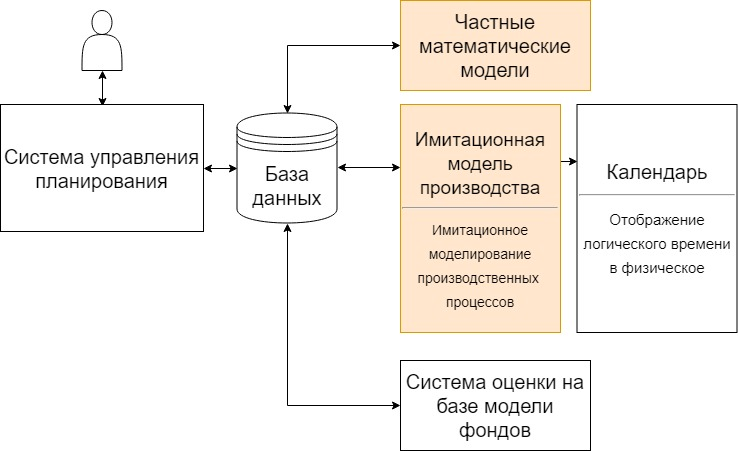
\includegraphics[width=1\linewidth]{fig/arh1.jpg}}
    \caption{Архитектура ПО}
    \label{ris:arh1}
\end{figure}

На рисунке \ref{ris:arh1} представлена архитектуры программного обеспечения. Данная архитектура содержит следующие элементы:

\begin{itemize}
    \item пользовательский интерфейс для взаимодействия с системой, который также позволяет получать информацию о работе системы в виде диаграмм, или графиков; 
    \item система управления планирования взаимодействует со всеми элементами системы и является главным распорядителем задач;
    \item база данных хранит всю информацию о производстве и результаты планирования; 
    \item основная задача имитационной модели заключается в построении оперативного расписания, в котором указаны все операции, время их начала и окончания, время начала и окончания участия производственных ресурсов в выполнения операций;
    \item календарь обрабатывает логические значения, используемые при планировании, и привязывает их к конкретным датам (физическое время);
    \item частные оптимизационные модели работают с входными данными имитационной модели. К этим данным применяются алгоритмы оптимизации, зависящие от конкретных целей. Таким целями могут быть: задачи упорядочивания, задачи согласования, задачи распределения, задачи с суммарными критериями оптимизации, задачи с минимаксимальными критериями оптимизации;
    \item модель оценки фондов работает с производственными мощностями и дают поверхностную оценку осуществимости заданного плана работы на такт (ПРТ), где ПРТ - это оперативный план на один такт сборочного производства, включающего в себя линии и посты, при полной его загрузке - заготовки находятся на каждом посту каждой линии; он обеспечивает максимизацию загрузки ресурсов (опционально - подбор необходимого количества ресурсов)
\end{itemize}

\section{Организация системы имитацонного моделирования}

\subsection{Формализация предметной области}

Для того, чтобы разрабатывать алгоритмы планирования в первую очередь необходимо формализовать предметную область. В данном случае формализуется сборочный цех со значимыми внутренними особенностями.

Как правило на любом предприятии имеется специальный документ – технологическая карта, детально описывающая весь перечень операций по достижению которых воспроизводится единица продукции. Технологическая карта хранит информацию о зависимостях между операциями, привязках ресурсов к операциям, трудоёмкостях операций, периодичность операций, результат каждой операции. 

Далее важно учесть ресурсы предприятия. В рамках сборочного производства такими ресурсами могут быть: персонал, оборудование, организация конвейерной производственной линии.

Последним пунктом для построения модели производства является производственный план. То есть перечень продукции в составе заказа и срок реализации данного заказа. На рисунке \ref{ris:Prod1} представлен пример взаимодействия перечисленных выше моделей. 

\begin{figure}[H]
    \center{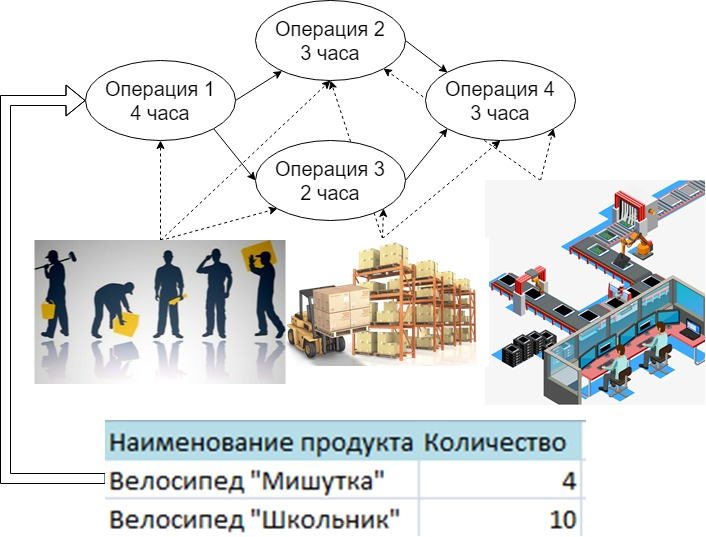
\includegraphics[width=1\linewidth]{fig/Prod1.jpg}}
    \caption{Модель производства}
    \label{ris:Prod1}
\end{figure}

\subsection{Математическое моделирование производственных процессов}

Для формализации процесса планирования в работе используются системы неравенств. Пример системы неравенств представлена на рисунке \ref{ris:sys1}. Система неравенств состоит из двух частей: статическую и динамическую. Статическая по своей сути описывает последовательность операций, описываемых в технологической карте. Динамическая рассчитывается во время планирования, которое включает ресурсные зависимости операций, поэтому последовательность определяется не только статической частью, но и динамической частью системы неравенств. 

\begin{figure}[H]
    \center{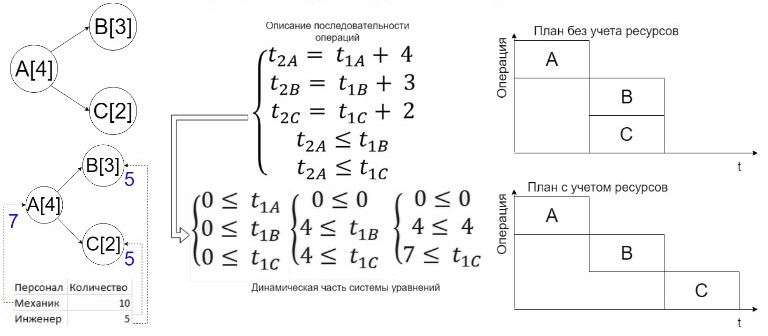
\includegraphics[width=1\linewidth]{fig/Screenshot_3.jpg}}
    \caption{Система неравенств}
    \label{ris:sys1}
\end{figure}

Таким образом планирование делится на шаги, каждый раз при этом формируются новые ограничения вводимые ресурсами.

По результатам анализа работы \cite{Jahangirian}, была составлена градация подходов к имитационному планированию представленная на рисунке \ref{ris:IM_detalApp}. 

Решение задачи планирования аналитическим подходом возможна, при этом основная проблема заключается в сложности реализации всех зависимостей, что делает данный подход сложным в исполнении.

Вторым решением задач имитационного моделирования является алгоритмический подход. Одним из примеров реализации данной идеи является Siemens Plant Simulation.

Система, разрабатываемая в рамках НИР, является гибридной моделью. Данный подход призван перенять лучшее у двух подходов. Там, где задачу можно решить аналитически использоваться аналитический подход, где задача приобретает большое количество зависимостей задача решается посредством алгоритмов. На рисунке \ref{ris:sys1} приведен пример, того, как выглядит математическая модель производственных процессов, где аналитически выведена статическая часть системы неравенств и посредством алгоритмов генерируется динамическая система неравенств.
\begin{figure}[H]
    \center{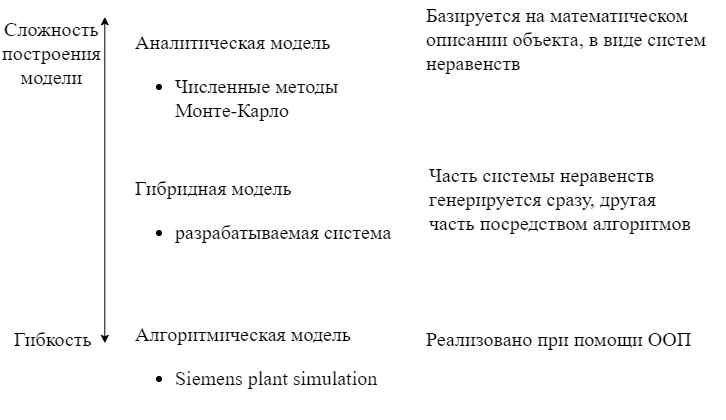
\includegraphics[width=1\linewidth]{fig/IM_detalApp.png}}
    \caption{Градация подходов к имитационному моделированию}
    \label{ris:IM_detalApp}
\end{figure}


\section{Частные оптимизационные модели}

В данном разделе приведено описание частных оптимизационных моделей. Необходимость применения данных моделей возникла, с появлением задач оптимизации на специфичных производствах. Данная специфика характеризуется уникальным для каждого предприятия структуры, где стандартные методы оптимизации будут не эффективны, либо не будут давать результата.

На текущий момент представлена одна частная оптимизационная модель, задача которой оптимизация сборочных производств. Сборочные производства характеризуются сборочными линиями, где на разных этапах установлены рабочие станции. Рабочий процесс на таком производстве выглядит следующим образом, загатовка перемещается от станции к станции, при этом на каждой станции ведется своя независимая работа.

Целью оптимиации является равномерная загрузка всех станций на линии, чтобы избежать простоя ресурсов производства. Для достижения данной цели были созданы модели необходимые для описания сборочного производства. Такими моделями являются ресурс рабочих, а также модель конвейера. Также разработаны методы оптимизации описанные в главе \ref{ALBP}.

\section{Выбор технологии реализации}

Планированию как вычислительному процессу необходимо большое количество вычислительных ресурсов и их грамотное использование. Это связано с тем фактом, что при планировании перебираются множество возможных вариантов и выбирается только один лучший (в данном случае имеются в виду алгоритмы оптимального поиска). Когда речь идет о возможности распараллеливания вычислительных ресурсов, требуется технология предоставляющая данную возможность. На данный момент практически все языки программирования имеют функцию распараллеливания, но языки, где это реализовано удобно и без изъянов, немного.  Для построения ядра моделирования был выбран многопоточный, компилируемый язык программирования - golang \cite{golangBook}.

Язык программирпования golang предоставляет следующие возможности:

\begin{itemize}
    \item [1)] Скорость обучения. Часто бывает, что разработчики имеют разный уровень подготовки, поэтому необходим язык который позволяет уменьшить затраты на изучения синтаксиса и как можно быстрее сосредоточиться на разработке. 
    \item [2)] Производительность. Golang компилируемый язык\cite{golangBook}. 
    \item [3)] Эффективность и возможность многопоточности. В Go есть горутины. Горутинами называют функцию, которая выполняется с другими гортинами в едином адресном пространстве. Основными преимуществами горутин являются: низкое потребление памяти, минимум накладных ресурсов на организацию, а также простота использования.
    \item [4)] Встроенный сборщик мусора.
\end{itemize}

Язык программирования golang вобрал преимущества низкоуровневых языков (сразу компилируется в двоичный код), а также высокоуровневых (имеет сборщик мусора для распределения и удаление объектов). Так как главный акцент, при выборе языка программирования, делался на производительность и поддержку многопоточности, golang является лучшим вариантом для создания ядра моделирования производственного плана. 

Данный акцент на быстроте и многопоточности был сделан не случайно. Как будет видно далее, в вопросах поиска оптимальных решений данные особенности golang будут очень востребованы.
\chapter{Система имитационного моделирования.}

\section{Назначение имитационной модели производственных процессов}

Основная задача имитационной модели заключается в построении расписания, в котором указаны все операции, время их начала и окончания, время начала и окончания участия производственных ресурсов в выполнения операций.

\subsection{Входные данные}
Некоторые из приведенных данных не учтены в текущей реализации, планируется добавление их в будущем. Эти данные \textit{помечены таким образом}.

\begin{itemize}
	\item ЦПВ - цеховая последовательность выпуска (выпуск продукции осуществляется в порядке, в котором они записаны в ЦПВ):
		\begin{itemize}
			\item наименование продукции;
			\item количество единиц продукции;	
			\item технологическая карта.
		\end{itemize}			
	\item Технологические карты, подробнее смотри (\ref{assembly_line_balancing:input_data}).
	\item Производственные ресурсы;
	\item \textit{Трафик доступности ресурсов};
	\item \textit{Структура цеха};
	\item \textit{Минимальное время участия ресурса в операции};
	\item \textit{Штрафы за переключение ресурса с одной операции на другую}. 
\end{itemize}

\subsection{Выходные данные}

\begin{itemize}
	\item Расчетные данные:	
		\begin{itemize}
			\item Перечень всех операций для всех единиц продукции ЦПВ;
			\item Время начала всех операций;
			\item Время окончания всех операций;
			\item \textit{Производственные ресурсы, привлекаемые к выполнению операции};
			\item \textit{Время начала и конца участия ресурса в операции};
			\item \textit{Загрузка производственных ресурсов}.
		\end{itemize}		
	\item Визуализиация данных пользователю:
		\begin{itemize}
			\item Расписания для производственных ресурсов;
			\item Диаграммы Ганта выпуска разных видов продукции;
			\item Визуализация загрузки производственных ресурсов.
		\end{itemize}		 
\end{itemize}


\section{Формализация предметной области}
Для того, чтобы разрабатывать алгоритмы планирования в первую очередь необходимо формализовать предметную область. В данном случае формализуется сборочный цех со значимыми внутренними особенностями.

Как правило на любом предприятии имеется специальный документ – технологическая карта, детально описывающая весь перечень операций по достижению которых воспроизводится единица продукции. Технологическая карта хранит информацию о зависимостях между операциями, привязках ресурсов к операциям, трудоёмкостях операций, периодичность операций, результат каждой операции. 

Далее важно учесть ресурсы предприятия. В рамках сборочного производства такими ресурсами могут быть: персонал, оборудование, организация конвейерной производственной линии.

Последним пунктом для построения модели производства является производственный план. То есть перечень продукции в составе заказа и срок реализации данного заказа. На рисунке \ref{ris:Prod1} представлен пример взаимодействия перечисленных выше моделей. 

\begin{figure}[H]
    \center{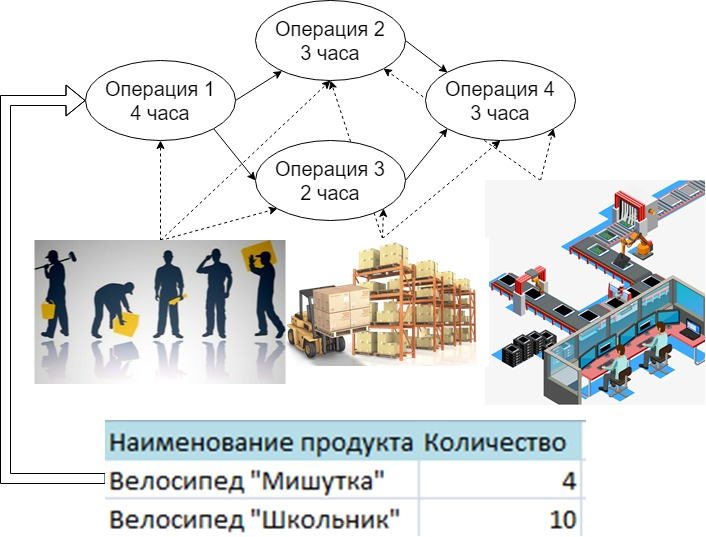
\includegraphics[width=1\linewidth]{fig/Prod1.jpg}}
    \caption{Модель производства}
    \label{ris:Prod1}
\end{figure}


\section{Математическое моделирование производственных процессов}

Для формализации процесса планирования в работе используются системы неравенств. Пример системы неравенств представлена на рисунке \ref{ris:sys1}. Система неравенств состоит из двух частей: статическую и динамическую. Статическая по своей сути копирует последовательность операций, описываемых в технологической карте. Динамическая накладывает дополнительные ограничения на систему неравенств, которая складывается из ресурсных зависимостей. Ресурсными зависимостями являются связи между операциями и фондом предприятия[3].

\begin{figure}[H]
    \center{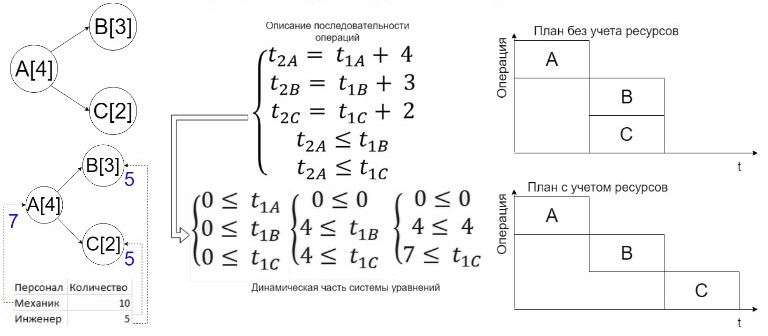
\includegraphics[width=1\linewidth]{fig/Screenshot_3.jpg}}
    \caption{Система неравенств}
    \label{ris:sys1}
\end{figure}

Таким образом планирование делится на шаги, каждый раз при этом формируются новые ограничения вводимые ресурсами[4].

\section{Предобработка технологических карт}

Одним из первых этапов работы алгоритма имитационного моделирования является подготовка входных данных. Входными данными имитационного моделирования являются: технологические карты, состав заказа, ресурсы предприятия, а также другие конфигурации.

На текущий момент реализована небольшая часть функционала отвечающую за предварительную обработку. Одной из таких функций является расчет длительности операций. Так как длительность операций является переменной величиной, зависимой от трудоемкости и количества людей выполняющих операцию, существует 4 настройки ресурса:

\begin{itemize}
    \item минимальная, при этом на операцию назначается минимальное количество людей, отсюда и длительность операции становится максимальной
    \item максимальная
    \item средняя
    \item случайная, данная конфигурация является частью работы эвристических алгоритмов, рассматриваемых в следующей главе
\end{itemize}

Также одной из возможностей предварительной настройки является алгоритм выбора операций последовательности(в тех случаях, когда позволяет причинно-следственная часть). На данный момент существует 2 конфигурации:

\begin{itemize}
    \item стандартная, при которой выбор осуществляется строго по порядку расположения в структурах данных
    \item случайная, при этом случайным образом выбирается одна из возможных операций, которые доступны в данный момент 
\end{itemize}

Возможность менять входные данные являются важным этапом обработки входных данных полученных из базы данных, позволяя при этом подготовить данные для дальнейшей обработки, а также гибко менять параметризуемые величины, чем и достигается большая вариативность, так необходимая для поиска оптимального значения. 

\section{Создание шаблона плана}

\section{Имитационное планирование}

\section{Оптимизация средствами имитацонного моделирования}

\subsubsection{Метод полного перебора}
Примером оптимизации может служить случайный выбор следующей операции при планировании, данный выбор возможен только в случаях одновременного выполнения нескольких независимых операций. Таким образом достигается вариативность при котором из разных реализаций, выбирается наилучший вариант. На рисунке (\ref{ris:Force}) изображены технологическая карта продукта и два плана, который были построены в результате случайного выбора операций. Как видно из рисунка (\ref{ris:Force}) первый план является более оптимальным по времени и ресурсам, чем второй.

\begin{figure}[H]
    \center{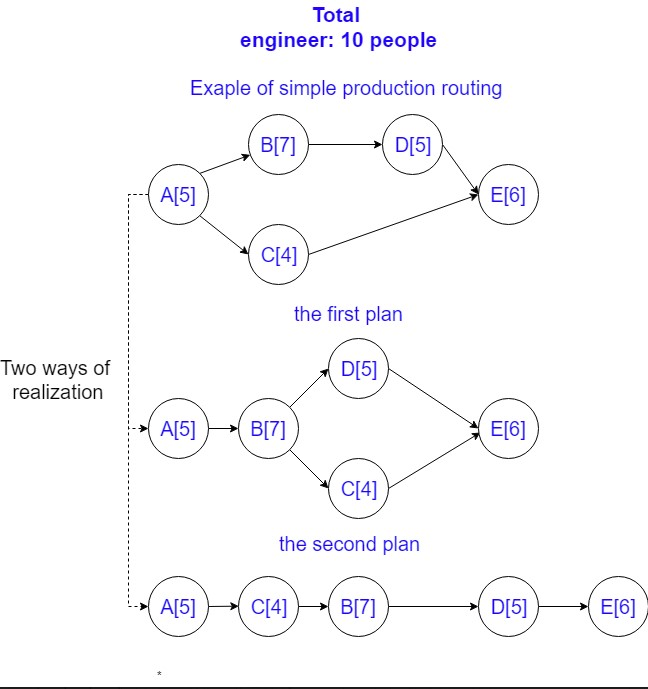
\includegraphics[width=1\linewidth]{fig/Force.jpg}}
    \caption{Два плана, полученные путем перебора исходной технологической карты}
    \label{ris:Force}
\end{figure}

\subsection{Методы оптимизации полного перебора}

\section{Результаты работы имитационной модели}
\chapter{Рассчет плана работы на такт.}

\section{Балансировка сборочной линии}

Производственная сборочная линия была впервые представлена
Генри Форд в начале 1900-х годов. Она была разработана, чтобы быть эффективным,
высокопроизводительным способом изготовления конкретного продукта. Базовая сборочная
линия состоит из набора рабочих станций, расположенных линейно, где каждая станция соединена погрузочно-разгрузочным устройством.
Основное движение материала по сборочной линии начинается с того, что деталь подается на первую станцию с
заданной скоростью подачи. Станция считается любой точкой на конвейере, в которой 
выполняется задание с заготовкой. Эти задачи могут выполняться машинами, роботами и
или людьми. Как только деталь поступает на станцию, то для нее выполняется задание, 
и деталь подается на следующую операцию. Время, необходимое для выполнения задачи
в каждой операции, называется временем процесса (Sury, 1971). Время цикла сборочной 
линии определяется желаемой производительностью. Этот уровень производства 
устанавливается таким образом, чтобы желаемое количество конечного продукта 
производилось в течение определенного периода времени (Baybars, 1986). Для того чтобы 
сборочная линия поддерживала определенную производительность, сумма времени обработки
на каждой станции не должна превышать время цикла на станциях (Fonseca et al, 2005). 
Если сумма времен обработки внутри станции меньше времени цикла, говорят, что на этой
станции присутствует время простоя (Erel et al, 1998). Одним из основных вопросов,
касающихся разработки сборочной линии, является порядок организации задач, которые 
необходимо выполнить. Для изготовления любого предмета есть несколько 
последовательностей задач, которые необходимо выполнить. Проблема балансировки 
сборочной линии (ALBP) возникла с изобретением сборочной линии. Хельгесон и др. 
(Helgeson и др., 1961) были первыми, кто предложил ALBP, а Сальвесон (Salveson, 1955)
был первым, кто опубликовал проблему в ее математической форме. 
Однако в течение первых сорока лет существования сборочной линии для балансировки
линий использовались только методы проб и ошибок (Erel et al., 1998). С тех пор 
было разработано множество методов для решения различных форм ALBP. 
Сальвесон (Salveson, 1955) сделал первую математическую попытку, решив задачу в
виде линейной программы. Гутьяр и Немхаузер (Gutjahr и Nemhauser, 1964) показали,
что проблема ALBP относится к классу NP-сложных задач комбинаторной оптимизации.
Это означает, что оптимальное решение не гарантируется для задач значительных размеров. 
Поэтому эвристические методы стали наиболее популярными методами решения проблемы.


Преимущества балансировки линии:

\begin{itemize}
    \item Минимизация количества рабочих станций при заданном цикле
    \item Минимизация цикла при заданном количестве рабочих станций
    \item Минимизация общего времени простоя
    \item Минимизация общего объекта или длины линии
\end{itemize}

Классификация проблемы ALB основана главным образом на целевых функциях и структуре проблемы. Различные версии проблем ALB представлены на рисунке (\ref{ris:image1}).

\begin{figure}[H]
    \center{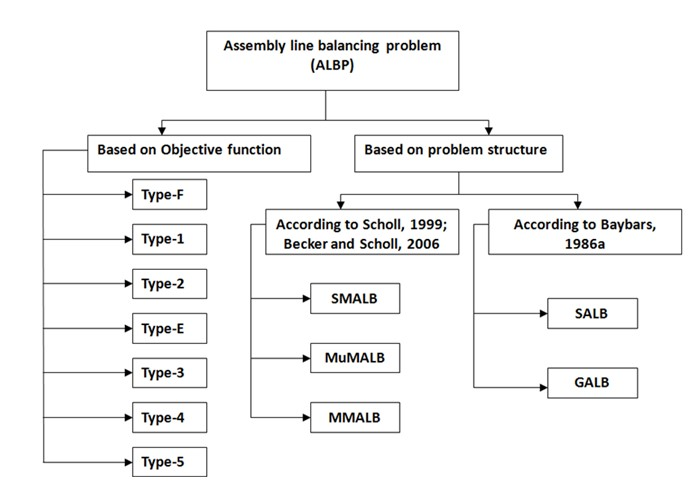
\includegraphics[width=1\linewidth]{fig/Screenshot_1.jpg}}
    \caption{Классификация ALBP}
    \label{ris:image1}
\end{figure}

\subsection{Проблемы базирующиеся на целевых функциях}
В данном подразделе рассматриваются целевые задачи балансировки линии. Далее перечисленные все обозримые проблемы приведенные на классификации \ref{ris:image1} и представленно их краткое описание.
\begin{itemize}
    \item Type F: Рассматривает возможность создание линии при заданном колличестве рабочих станций и цикле.
    \item Type 1: Рассматривает задачу минимизации количества рабочих станций, при фиксированном времени цикла.
    \item Type 2: Рассматривает задачу минимизации времени цикла, при фиксированном количестве рабочих станций.
    \item Type E: Данный тип является самой общей версией ПРТ и рассматривает получение максимальной эффективности линии при минимальном цикле и количестве станций.
    \item Type 3: Рассматривает задачу максимизации плавности рабочей нагрузки.
    \item Type 4: Рассматривают максимизацию рабочей связанности, используется для быстрого производства однотипного продукта.
    \item Type 5: Рассматривает типы 3 и 4 для нескольких продуктов
\end{itemize}

В рамках данной работы рассматривается функция повышения эффективности загрузки. Эффективность сборочной линии подразумевает равную загрузку всех рабочих станций на сборочной линии. 

\subsection{Проблемы основывающиеся на структуре линии}
В данном разделе рассматриваются структурные задачи балансировки линии. Далее перечислены структурные проблемы приведенные на рисунке (\ref{ris:image1}) и их описание.

\begin{itemize}
    \item SMALB: Данная проблема затрагивает структуру, когда на линии производится один тип продукта
    \item MuMALBP: Затрагивает проблемы производства более одного типа продукта партиями на одной линии
    \item MMALBP: Затрагивает производство разных типов продуктов на одной линии в любом порядке, без времени переключения (имется ввиду переключение на производство другого типа продукта)
\end{itemize}

\begin{figure}[H]
    \center{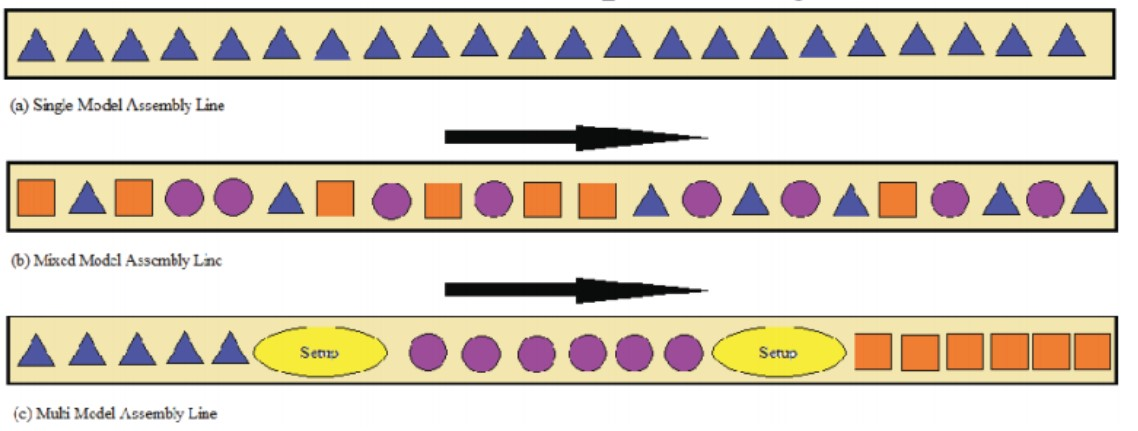
\includegraphics[width=1\linewidth]{fig/Screenshot_2.jpg}}
    \caption{Структура линий из классификации, изображенной на рисунке \ref{ris:image1}}
    \label{ris:shapeOfLines}
\end{figure}

Созданная имитационная модель позволяет игнорировать структурные особенности линии. Основные ограничения, которые невозможно игнорировать включены в технологическую карту. 
\todo[inline, color=red]{Пока непонятно куда девать время предустановки линии в случае MMALBP}

Источник: https://ru.scribd.com/doc/7699063/Introduction-of-Line-Balancing



\section{Обзоры методов решения проблем балансировки линии}

На текущий момент известны множество подходов решения проблемы балансировки линии. Наиболее популярные подходы и методы приведены на рисунке (\ref{ris:Approaches}).

\begin{figure}[H]
    \center{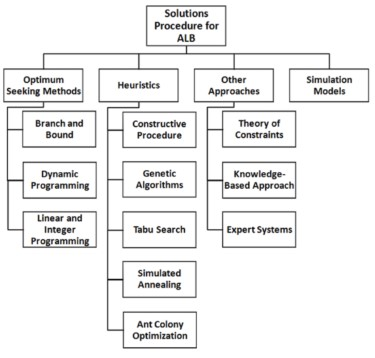
\includegraphics[width=1\linewidth]{fig/Approaches.jpg}}
    \caption{Различные процедуры решения для ALB}
    \label{ris:Approaches}
\end{figure}

Методы оптимального поиска основаны на математических подходах и позволяют найти из множества объектов оптимальный, который соответствует заданным критериям. Одной из основных проблем данного подхода является вычислительная сложность, что в контексте поиска наилучшей конфигурации конвейера, приводит к существенному ограничению использования методов оптимального поиска.

Методы эвристики позволяют избежать проблемы комбинаторной сложности задачи, но при этом результат не всегда будет являться самым оптимальным из возможных. Также эффективность работы алгоритмов эвристики во многом зависят от подхода. На рисунке (\ref{ris:Approaches}) приведены 5 различных эвристических алгоритмов, которые использовались для решения проблемы балансировки линии. Наиболее эффективным из данной группы показал себя генетический алгоритм поиска(ссылка на пруфы). Рассмотрим подробно, как работает генетический алгоритм в контексте балансировки линии.

\subsection{Генетический алгоритм}

Генетические алгоритмы хорошо подходят для решения задач планирования производства, потому что в отличие от эвристических методов генетические алгоритмы работают на совокупности решений, а не на одном решении. В производственном планировании эта совокупность решений состоит из множества ответов, которые могут иметь разные, иногда противоречивые цели. Например, в одном решении оптимизировать производственный процесс, который будет завершен за минимальное время. В другом решении оптимизировать для минимального количества дефектов.

По мере того как увеличиваются количество целей, которые пытаемся достичь, также увеличивается количество ограничений на проблему и аналогичным образом увеличиваем сложность. Генетические алгоритмы идеальны для задач такого типа, когда пространство поиска велико, а количество возможных решений мало.

Чтобы применить генетический алгоритм к задаче планирования, необходимо сначала представить каким образом обозначить геном. Одним из способов представления генома планирования является определение последовательности задач и времени начала этих задач относительно друг друга. Каждое задание и соответствующее время его запуска представляют собой ген.

Определенная последовательность задач и времени начала (гены) представляет один ген в нашей популяции. Чтобы убедиться, что геном является возможным решением, надо чтобы он соответствовал ограничениям приоритета. Далее генерируется начальная популяция, используя случайные времена начала в пределах ограничений предшествования. С помощью генетических алгоритмов берется начальная популяция и скрещивается, комбинируя гены с небольшим количеством случайности (мутации). Потомки этой комбинации выбираются на основе фитнес-функции, которая включает одно или много наших ограничений, таких как минимизация времени и минимизация дефектов. Данный процесс продолжаться либо в течение заранее выделенного времени, либо до тех пор, пока не найдется решение, которое соответствует минимальным критериям. В целом каждое последующее поколение будет иметь более высокую среднюю пригодность, то есть займет меньше времени с более высоким качеством, чем предыдущие поколения. При планировании задач, как и в случае с другими решениями генетического алгоритма, необходимо убедиться, что мы не выбираются недопустимые потомки, такие как отпрыски, которые нарушают наше ограничение приоритета. Также может потребоваться добавить дополнительные значения пригодности, такие как минимизация затрат; однако каждое добавляемое ограничение значительно увеличивает пространство поиска и уменьшает количество подходящих решений.

\likechapter{Заключение}
Цель достигнута, задачи выполнены %Сам диплом

%%%%%%%%%%%%%%%%%%%%%%%%%%%%%%%%%%%%%%%%%%
% НАЧАЛО ТЕКСТА	
	% Тут можно начинать писать текст.

	\chapter{Глава}
\label{cha:chapter}

\todo[inline, color=red]{так выглядит заметка в тексте}
\section{Новый раздел}

\subsection{Оформление текста}
Пустая строка

- это новый абзац\\%\\ - интервал между строками

\textbf{Жирный}

\textit{Курсив}

\sout{Зачерктунтый}

\textcolor{red}{Красный}\\

Перечисление без нумерации
\begin{itemize}
	\item Первый
	\begin{itemize}
		\item 1-1
		\item 1-2
	\end{itemize}
	\item Второй\\
\end{itemize}

Перечисление с нумерацией

\begin{enumerate}
	\item Первый
	\item Второй\\
\end{enumerate}

Ссылка на литературу\todo[color=green]{Заметка на полях} \cite{Pup09}.

\subsection{Таблица}


\begin{table}[h]
	\caption{\label{tab:canonsummary}Измерительные характеристики цифровой камеры Canon EOS 400D.} %Заголовок
	\begin{center}%по центру
		\begin{tabular}{|c|c|} % два столбца с границами и выравниванием по центру
			\hline % горизонтальная граница
			% Первая строка, "&" - hfpltkbntkm cnjk.wjd
			Параметр 		& 		Значение \\
			\hline
			Разрешение		 & $3888 \times 2592$ \\
			Размер сенсора	 & $22.2 \times 14.8$ мм \\
			АЦП & 12~bit\\
			\hline
			\multicolumn{2}{|c|}{Результаты измерений} \\ % Объединяем столбцы с выравниванием по центру
			\hline
			Темновое смещение (BLO) & 256 \\
			Максимальный линейный сигнал & 3070~DN \\
			Значение насыщения & 3470~DN \\
			\hline
		\end{tabular}
	\end{center}
\end{table}


\subsection{Формулы}
Формула или математическое выражение в тексте $a=b$

Формула или математическое выражение
$$
a=b+c
$$
с отдельной строки.\\

Горизонтальный $b\: a$ пробел

Толстый горизонтальный $c\;e$ пробел

Индексы $a_b^c$

Нумерованные формулы
\begin{eqnarray}
\label{eq:a}%ссылка на формулу
a=b+c
\end{eqnarray}

Так ссылаться на формулу, рисунок или таблицу в тексте (\ref{eq:a})

Формула в несколько строк
\begin{eqnarray*}
\label{new_formula}
&a=b,\\
&c=e
\end{eqnarray*}

$$
\alpha,  \theta, \upsilon, \beta, \vartheta, \pi, \phi, \gamma, \iota, \varpi, \varphi,
, \delta , \kappa , \rho , \chi
, \epsilon , \lambda , \varrho , \psi
, \varepsilon , \mu , \sigma , \omega
, \zeta , \nu , \varsigma
, \eta, \xi , \tau
$$

\subsection{Рисунки}
\begin{figure}[H]
	\center{
\includegraphics[width=1\linewidth]{fig/fig.jpeg}}
	\caption{Зависимость сигнала от шума для данных.}
	\label{ris:image}
\end{figure}

Сылка на рисунок \ref{ris:image}.


\begin{lstlisting}[style=pseudocode,caption={Алгоритм оценки дипломных работ}]
def EvaluateDiplomas():
	for each student in Masters:
		student.Mark := 5
	for each student in Engineers:
		if Good(student):
			student.Mark := 5
		else:
			student.Mark := 4
\end{lstlisting}


%%% Local Variables:
%%% mode: latex
%%% TeX-master: "rpz"
%%% End:
 % Начинается с новой страницы, так как содержит Главу (Chapter).
% КОНЕЦ ТЕКСТА
%%%%%%%%%%%%%%%%%%%%%%%%%%%%%%%%%%%%%%%%%%

\bibliographystyle{ugost2008}
\bibliography{bibl}


\end{document}
